\documentclass[10pt,a4paper]{ctexart}
\usepackage[margin=2cm]{geometry}
\usepackage{graphicx}
\usepackage{float}      % 支持 [H] 浮动体选项
\usepackage{hyperref}
\usepackage{amsmath}    % 提供方程环境
\usepackage{physics}    % 简化向量、微分算子语法
\newcommand{\myspace}[1]{\par\vspace{#1\baselineskip}} %自定义空一行
\usepackage{fancyhdr}
\pagestyle{fancy}
\fancyhf{}  % 清除所有页眉页脚
\fancyfoot[C]{\thepage}  % 在页脚中央设置页码
\renewcommand{\headrulewidth}{0pt}  % 去掉页眉横线
\renewcommand{\footrulewidth}{0pt}  % 去掉页脚横线

\usepackage{hyperref}
\hypersetup{
    colorlinks=true,
    linkcolor=blue,
    filecolor=magenta,      
    urlcolor=cyan,
    pdftitle={Overleaf Example},
    pdfpagemode=FullScreen,
    }

\usepackage{titlesec}

% 重新定义section格式
\titleformat{\section}
  {\normalfont\Large\bfseries}
  {\chinese{section}、}
  {0pt}
  {}

% 给出常用字号的自定义指令
\newcommand{\chuhao}{\fontsize{42pt}{48pt}\selectfont}
\newcommand{\xiaochu}{\fontsize{36pt}{42pt}\selectfont}
\newcommand{\xiaoer}{\fontsize{18pt}{21.6pt}\selectfont}
\newcommand{\sanhao}{\fontsize{16pt}{20pt}\selectfont}
\newcommand{\xiaosan}{\fontsize{15pt}{18pt}\selectfont}
\newcommand{\sihao}{\fontsize{14pt}{18pt}\selectfont}
\newcommand{\xiaosi}{\fontsize{12pt}{16pt}\selectfont}
\newcommand{\wuhao}{\fontsize{10.5pt}{12.6pt}\selectfont}

% 定义中文数字转换
\titleformat{\section}
  {\normalfont\Large\bfseries}
  {\zhnum{section}、}  % 使用\zhnum而不是\chinese
  {0pt}
  {}

% 标题设置
\title{\xiaochu\textbf{物理实验预习报告}}
\author{}
\date{}

\begin{document}

\vspace*{36pt} % 顶部空白

% 居中填写区域
\begin{center}   
    \xiaochu\textbf{物理实验预习报告}
    % 预留空白区域
    \vspace{13pt}
    \vspace{13pt}
    \vspace{13pt}
    \vspace{13pt}
    
    \sanhao\textbf{实验名称：\underline{\makebox[10cm]{ 用双臂电桥测低电阻}}} \\[10pt]
    \sanhao\textbf{指导教师：\underline{\makebox[10cm]{ 刘公羽 }}} \\[30pt]
    
    % 预留空白区域
    \myspace{6}
    
   \sihao\textbf{班级：\underline{\makebox[6cm]{}}} \\[10pt]
    \sihao\textbf{姓名：\underline{\makebox[6cm]{}}} \\[10pt]
    \sihao\textbf{学号：\underline{\makebox[6cm]{}}} \\[30pt]
    
   \sihao\textbf{实验日期: 
   \underline{\makebox[0.8cm]{2025}}  年 
   \underline{\makebox[0.4cm]{12}}月
   \underline{\makebox[0.4cm]{17}}日  
   星期\underline{\makebox[0.6cm]{三}}上午}
    
    \vspace{18pt}
    \sihao 浙江大学物理实验教学中心
    
\end{center}

\newpage

    \section{实验综述}
    
    \xiaosi （自述实验现象、实验原理和实验方法，不超过300字，5分）

    r1和r2代表接触电阻和导线电阻，一般在0.01-1 Ω的数量级。
    由图可见，当测量电阻时r1和r2会包含于内，实际测得的阻值为Rx+r1+r2，当Rx与r1、r2同数量级时引入的误差就很大。
\begin{figure}[H]
        \centering
        
\includegraphics[width=0.8\textwidth]{figure/circuit.png}
        \caption{接触电阻影响示意图}
    \end{figure}

    因此发明了双臂电桥测电阻的办法。等效电路如图
    \begin{figure}[H]
        \centering
        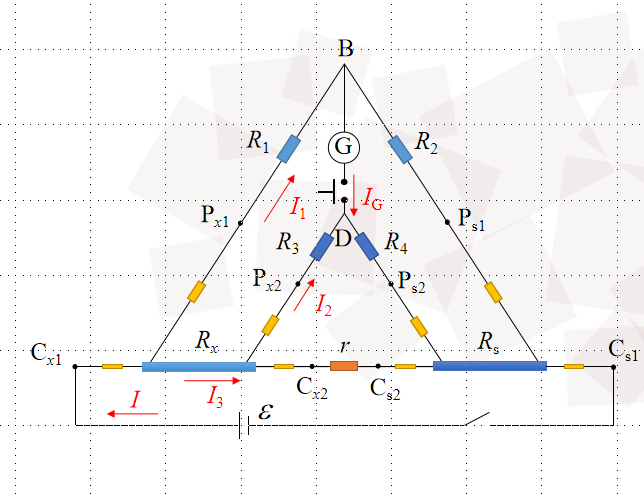
\includegraphics[width=0.8\textwidth]{figure/bridge.png}
        \caption{双臂电桥电路图}
    \end{figure}
    根据基尔霍夫定律可以得到，在$\frac{R_1}{R_2}=\frac{R_3}{R_4}$时$R_x=\frac{R_1}{R_2}R_s$

    室温下温度变化不大时金属温阻表现为线性$R_t=R_0(1+\alpha t)$。

    利用双臂电桥法测量电阻，改变温度，就可以绘制金属电阻-温度曲线，测量温度系数。
\myspace{2}
    
    \section{实验重点}
    
    \xiaosi（简述本实验的学习重点，不超过100字，3分）

掌握双臂电桥测量低电阻的原理和使用方法

了解单臂电桥与双臂电桥的关系和区别

    \myspace{2}
    
    \section{实验难点}

    \xiaosi（简述本实验的实现难点，不超过100字，2分）

    准确控制温度。温度不易控制，且达到设定温度后会有惯性或者冷却，需要迅速完成对应的实验操作。

    准确测量金属电阻的直径、长度等参数。
\myspace{2}


\newpage

\sihao\textbf{注意事项：}
\xiaosi
\begin{enumerate}
    \item 用PDF格式上传“预习报告”，文件名：学生姓名+学号+实验名称+周次。
    \item “预习报告”必须递交在“学在浙大”的本课程的对应实验项目的“作业”模块内。
    \item “预习报告”还须拷贝到“实验报告”中（便以教师批改）。
    \item 大学物理实验”课程选做实验使用本“预习报告”；必做实验无须写预习报告，前往“学在浙大”完成预习测试即可。
\end{enumerate}

\vspace{1cm}
\xiaosi\centering \textbf{浙江大学物理实验教学中心制}

\end{document}
